\begin{frame}
\frametitle{Exemples}
\framesubtitle{Apparition d'une figure}

On peut aussi mettre du texte brut avant apparition d'une figure

\visible<2-> {% On n'utilise pas "\onslide" ici car on ne peut pas régler le niveau de transparence de la figure
\begin{center}
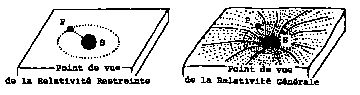
\includegraphics[width=0.5\linewidth]{figures/Fig02}
\end{center}
} % NB: \visible rend visible son argument, c'est-à-dire qu'il faut mettre ce 
  % qu'on veut rendre visible entre accolades par la suite contrairement à \onslide
  % qui joue le rôle d'une bascule.

\onslide<3->
Et le texte qui suit

\end{frame}
